\begin{frame}\frametitle{Session Types: Intro}
What are Session Types?
\begin{itemize}
\item Type discipline for specifying protocols in communication-intensive systems(e.g. multi-core programming, mobile applications, or web services)
% \item Formalism to model protocols in distributed systems
\item Introduced more than 20 years ago by~\cite{honda93, takeuchi94, honda98}
\item Guarantee properties such as privacy, communication safety and session fidelity
\item At runtime communication follows the protocol
\item Significant theme in programming languages
\end{itemize}

\end{frame}

\begin{frame}\frametitle{Session Types: Example}

  \begin{figure}[htb]
    \centering
    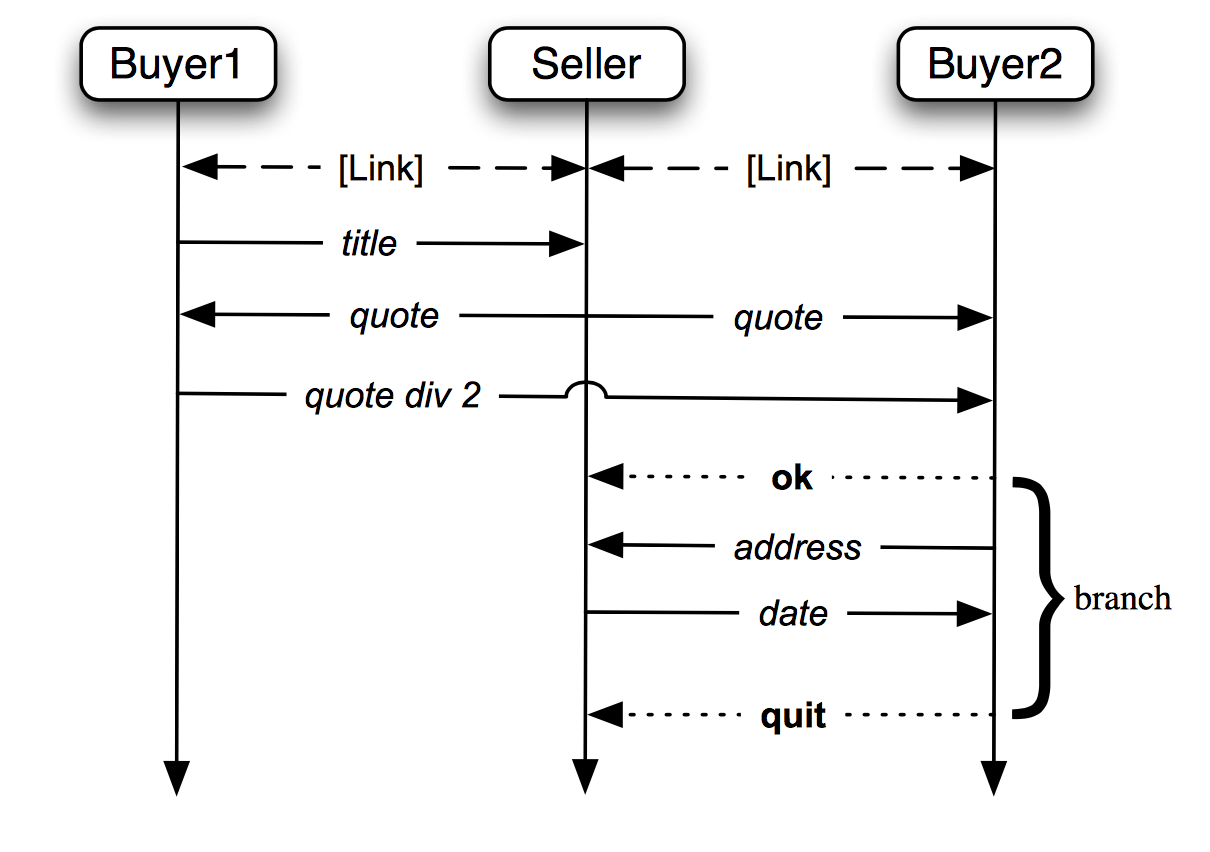
\includegraphics[scale=0.45]{examples/TwoBuyer.png}
    \caption{Two Buyer Protocol~\cite{honda2008multiparty}}
  \end{figure}
\end{frame}
%First Buyer1 sends a book title to Seller, then Seller sends back a quote to Buyer1/2; Buyer1 now tells Buyer2 how much she can contribute, and Buyer2 notifies Seller if it accepts the quote or not.

\begin{frame}[fragile]\frametitle{Session Types: Example}
  \begin{lstlisting}
  global protocol TwoBuyer(role Buyer1, role Buyer2,
  role Seller) {
    book(title) from Buyer1 to Seller;
    book(quote) from Seller to Buyer1, Buyer2;
    contribution(quote) from Buyer1 to Buyer2;
    choice at Buyer2 {
      ok from Buyer2 to Seller;
      deliver(address) from Buyer2 to Seller;
      deliver(date) from Seller to Buyer2;
      } or {
      quit from Buyer2 to Seller;
      }
      }
  \end{lstlisting}\footnote{written in Scribble, a protocol description language that can describe how two or more participating entities interact should interact with each other \url{www.scribble.org}}
  ~\cite{honda2008multiparty}
\end{frame}
